% Options for packages loaded elsewhere
\PassOptionsToPackage{unicode}{hyperref}
\PassOptionsToPackage{hyphens}{url}
\PassOptionsToPackage{dvipsnames,svgnames,x11names}{xcolor}
%
\documentclass[
  letterpaper,
  DIV=11,
  numbers=noendperiod]{scrartcl}

\usepackage{amsmath,amssymb}
\usepackage{iftex}
\ifPDFTeX
  \usepackage[T1]{fontenc}
  \usepackage[utf8]{inputenc}
  \usepackage{textcomp} % provide euro and other symbols
\else % if luatex or xetex
  \usepackage{unicode-math}
  \defaultfontfeatures{Scale=MatchLowercase}
  \defaultfontfeatures[\rmfamily]{Ligatures=TeX,Scale=1}
\fi
\usepackage{lmodern}
\ifPDFTeX\else  
    % xetex/luatex font selection
\fi
% Use upquote if available, for straight quotes in verbatim environments
\IfFileExists{upquote.sty}{\usepackage{upquote}}{}
\IfFileExists{microtype.sty}{% use microtype if available
  \usepackage[]{microtype}
  \UseMicrotypeSet[protrusion]{basicmath} % disable protrusion for tt fonts
}{}
\makeatletter
\@ifundefined{KOMAClassName}{% if non-KOMA class
  \IfFileExists{parskip.sty}{%
    \usepackage{parskip}
  }{% else
    \setlength{\parindent}{0pt}
    \setlength{\parskip}{6pt plus 2pt minus 1pt}}
}{% if KOMA class
  \KOMAoptions{parskip=half}}
\makeatother
\usepackage{xcolor}
\setlength{\emergencystretch}{3em} % prevent overfull lines
\setcounter{secnumdepth}{-\maxdimen} % remove section numbering
% Make \paragraph and \subparagraph free-standing
\makeatletter
\ifx\paragraph\undefined\else
  \let\oldparagraph\paragraph
  \renewcommand{\paragraph}{
    \@ifstar
      \xxxParagraphStar
      \xxxParagraphNoStar
  }
  \newcommand{\xxxParagraphStar}[1]{\oldparagraph*{#1}\mbox{}}
  \newcommand{\xxxParagraphNoStar}[1]{\oldparagraph{#1}\mbox{}}
\fi
\ifx\subparagraph\undefined\else
  \let\oldsubparagraph\subparagraph
  \renewcommand{\subparagraph}{
    \@ifstar
      \xxxSubParagraphStar
      \xxxSubParagraphNoStar
  }
  \newcommand{\xxxSubParagraphStar}[1]{\oldsubparagraph*{#1}\mbox{}}
  \newcommand{\xxxSubParagraphNoStar}[1]{\oldsubparagraph{#1}\mbox{}}
\fi
\makeatother

\usepackage{color}
\usepackage{fancyvrb}
\newcommand{\VerbBar}{|}
\newcommand{\VERB}{\Verb[commandchars=\\\{\}]}
\DefineVerbatimEnvironment{Highlighting}{Verbatim}{commandchars=\\\{\}}
% Add ',fontsize=\small' for more characters per line
\usepackage{framed}
\definecolor{shadecolor}{RGB}{241,243,245}
\newenvironment{Shaded}{\begin{snugshade}}{\end{snugshade}}
\newcommand{\AlertTok}[1]{\textcolor[rgb]{0.68,0.00,0.00}{#1}}
\newcommand{\AnnotationTok}[1]{\textcolor[rgb]{0.37,0.37,0.37}{#1}}
\newcommand{\AttributeTok}[1]{\textcolor[rgb]{0.40,0.45,0.13}{#1}}
\newcommand{\BaseNTok}[1]{\textcolor[rgb]{0.68,0.00,0.00}{#1}}
\newcommand{\BuiltInTok}[1]{\textcolor[rgb]{0.00,0.23,0.31}{#1}}
\newcommand{\CharTok}[1]{\textcolor[rgb]{0.13,0.47,0.30}{#1}}
\newcommand{\CommentTok}[1]{\textcolor[rgb]{0.37,0.37,0.37}{#1}}
\newcommand{\CommentVarTok}[1]{\textcolor[rgb]{0.37,0.37,0.37}{\textit{#1}}}
\newcommand{\ConstantTok}[1]{\textcolor[rgb]{0.56,0.35,0.01}{#1}}
\newcommand{\ControlFlowTok}[1]{\textcolor[rgb]{0.00,0.23,0.31}{\textbf{#1}}}
\newcommand{\DataTypeTok}[1]{\textcolor[rgb]{0.68,0.00,0.00}{#1}}
\newcommand{\DecValTok}[1]{\textcolor[rgb]{0.68,0.00,0.00}{#1}}
\newcommand{\DocumentationTok}[1]{\textcolor[rgb]{0.37,0.37,0.37}{\textit{#1}}}
\newcommand{\ErrorTok}[1]{\textcolor[rgb]{0.68,0.00,0.00}{#1}}
\newcommand{\ExtensionTok}[1]{\textcolor[rgb]{0.00,0.23,0.31}{#1}}
\newcommand{\FloatTok}[1]{\textcolor[rgb]{0.68,0.00,0.00}{#1}}
\newcommand{\FunctionTok}[1]{\textcolor[rgb]{0.28,0.35,0.67}{#1}}
\newcommand{\ImportTok}[1]{\textcolor[rgb]{0.00,0.46,0.62}{#1}}
\newcommand{\InformationTok}[1]{\textcolor[rgb]{0.37,0.37,0.37}{#1}}
\newcommand{\KeywordTok}[1]{\textcolor[rgb]{0.00,0.23,0.31}{\textbf{#1}}}
\newcommand{\NormalTok}[1]{\textcolor[rgb]{0.00,0.23,0.31}{#1}}
\newcommand{\OperatorTok}[1]{\textcolor[rgb]{0.37,0.37,0.37}{#1}}
\newcommand{\OtherTok}[1]{\textcolor[rgb]{0.00,0.23,0.31}{#1}}
\newcommand{\PreprocessorTok}[1]{\textcolor[rgb]{0.68,0.00,0.00}{#1}}
\newcommand{\RegionMarkerTok}[1]{\textcolor[rgb]{0.00,0.23,0.31}{#1}}
\newcommand{\SpecialCharTok}[1]{\textcolor[rgb]{0.37,0.37,0.37}{#1}}
\newcommand{\SpecialStringTok}[1]{\textcolor[rgb]{0.13,0.47,0.30}{#1}}
\newcommand{\StringTok}[1]{\textcolor[rgb]{0.13,0.47,0.30}{#1}}
\newcommand{\VariableTok}[1]{\textcolor[rgb]{0.07,0.07,0.07}{#1}}
\newcommand{\VerbatimStringTok}[1]{\textcolor[rgb]{0.13,0.47,0.30}{#1}}
\newcommand{\WarningTok}[1]{\textcolor[rgb]{0.37,0.37,0.37}{\textit{#1}}}

\providecommand{\tightlist}{%
  \setlength{\itemsep}{0pt}\setlength{\parskip}{0pt}}\usepackage{longtable,booktabs,array}
\usepackage{calc} % for calculating minipage widths
% Correct order of tables after \paragraph or \subparagraph
\usepackage{etoolbox}
\makeatletter
\patchcmd\longtable{\par}{\if@noskipsec\mbox{}\fi\par}{}{}
\makeatother
% Allow footnotes in longtable head/foot
\IfFileExists{footnotehyper.sty}{\usepackage{footnotehyper}}{\usepackage{footnote}}
\makesavenoteenv{longtable}
\usepackage{graphicx}
\makeatletter
\def\maxwidth{\ifdim\Gin@nat@width>\linewidth\linewidth\else\Gin@nat@width\fi}
\def\maxheight{\ifdim\Gin@nat@height>\textheight\textheight\else\Gin@nat@height\fi}
\makeatother
% Scale images if necessary, so that they will not overflow the page
% margins by default, and it is still possible to overwrite the defaults
% using explicit options in \includegraphics[width, height, ...]{}
\setkeys{Gin}{width=\maxwidth,height=\maxheight,keepaspectratio}
% Set default figure placement to htbp
\makeatletter
\def\fps@figure{htbp}
\makeatother

\KOMAoption{captions}{tableheading}
\usepackage{xcolor}
\makeatletter
\@ifpackageloaded{tcolorbox}{}{\usepackage[skins,breakable]{tcolorbox}}
\@ifpackageloaded{fontawesome5}{}{\usepackage{fontawesome5}}
\definecolor{quarto-callout-color}{HTML}{909090}
\definecolor{quarto-callout-note-color}{HTML}{0758E5}
\definecolor{quarto-callout-important-color}{HTML}{CC1914}
\definecolor{quarto-callout-warning-color}{HTML}{EB9113}
\definecolor{quarto-callout-tip-color}{HTML}{00A047}
\definecolor{quarto-callout-caution-color}{HTML}{FC5300}
\definecolor{quarto-callout-color-frame}{HTML}{acacac}
\definecolor{quarto-callout-note-color-frame}{HTML}{4582ec}
\definecolor{quarto-callout-important-color-frame}{HTML}{d9534f}
\definecolor{quarto-callout-warning-color-frame}{HTML}{f0ad4e}
\definecolor{quarto-callout-tip-color-frame}{HTML}{02b875}
\definecolor{quarto-callout-caution-color-frame}{HTML}{fd7e14}
\makeatother
\makeatletter
\@ifpackageloaded{caption}{}{\usepackage{caption}}
\AtBeginDocument{%
\ifdefined\contentsname
  \renewcommand*\contentsname{Table of contents}
\else
  \newcommand\contentsname{Table of contents}
\fi
\ifdefined\listfigurename
  \renewcommand*\listfigurename{List of Figures}
\else
  \newcommand\listfigurename{List of Figures}
\fi
\ifdefined\listtablename
  \renewcommand*\listtablename{List of Tables}
\else
  \newcommand\listtablename{List of Tables}
\fi
\ifdefined\figurename
  \renewcommand*\figurename{Figure}
\else
  \newcommand\figurename{Figure}
\fi
\ifdefined\tablename
  \renewcommand*\tablename{Table}
\else
  \newcommand\tablename{Table}
\fi
}
\@ifpackageloaded{float}{}{\usepackage{float}}
\floatstyle{ruled}
\@ifundefined{c@chapter}{\newfloat{codelisting}{h}{lop}}{\newfloat{codelisting}{h}{lop}[chapter]}
\floatname{codelisting}{Listing}
\newcommand*\listoflistings{\listof{codelisting}{List of Listings}}
\makeatother
\makeatletter
\makeatother
\makeatletter
\@ifpackageloaded{caption}{}{\usepackage{caption}}
\@ifpackageloaded{subcaption}{}{\usepackage{subcaption}}
\makeatother

\ifLuaTeX
  \usepackage{selnolig}  % disable illegal ligatures
\fi
\usepackage{bookmark}

\IfFileExists{xurl.sty}{\usepackage{xurl}}{} % add URL line breaks if available
\urlstyle{same} % disable monospaced font for URLs
\hypersetup{
  pdftitle={Homework 4},
  pdfauthor={Sarah E. Grabinski},
  colorlinks=true,
  linkcolor={blue},
  filecolor={Maroon},
  citecolor={Blue},
  urlcolor={Blue},
  pdfcreator={LaTeX via pandoc}}


\title{Homework 4}
\usepackage{etoolbox}
\makeatletter
\providecommand{\subtitle}[1]{% add subtitle to \maketitle
  \apptocmd{\@title}{\par {\large #1 \par}}{}{}
}
\makeatother
\subtitle{Answer Key}
\author{Sarah E. Grabinski}
\date{2024-11-16}

\begin{document}
\maketitle

\renewcommand*\contentsname{Table of contents}
{
\hypersetup{linkcolor=}
\setcounter{tocdepth}{3}
\tableofcontents
}

\section*{Instructions}\label{instructions}
\addcontentsline{toc}{section}{Instructions}

\emph{You work for Secretary of Transportation Pete Buttigieg, and he
has asked you to prepare a year end report comparing flight delays
during the Trump administration and the Biden administration. He would
like to know on average what percentage of flights were delayed and how
long they were delayed for during each administration. He would also
know if there was a meaningful difference between the two
administrations.}

\emph{Your data comes from the
\href{https://www.transtats.bts.gov/OT_Delay/OT_DelayCause1.asp?20=E}{Bureau
of Transportation Statistics}, run by the US Department of
Transportation. It is a random sample of 800 airports from the years
2016-2024.}

\begin{itemize}
\item
  Follow the previously given instructions to start a new project in
  RStudio for Homework 4. Go to the project folder.
\item
  Download the files \texttt{homework4\_template.qmd} and
  \texttt{airline\_delays.xlsx} from Canvas. Move these files to your
  Homework 4 project folder.
\item
  Please save your homework as
  \texttt{homework4\_firstnamelastname.qmd}. When you render, it should
  produce the file \texttt{homework4\_firstnamelastname.html}.
\item
  Follow the prompts to complete the steps of each statistical analysis.
  Work must be shown in code chunks for partial credit.
\item
  Add packages to the \texttt{load\_packages} code chunk as you work
  through the analysis and need their functions. This portion has not
  been pre-filled for you.
\item
  Answer in complete sentences where indicated.
\end{itemize}

\section*{Codebook}\label{codebook}
\addcontentsline{toc}{section}{Codebook}

\begin{longtable}[]{@{}
  >{\raggedright\arraybackslash}p{(\columnwidth - 4\tabcolsep) * \real{0.3333}}
  >{\raggedright\arraybackslash}p{(\columnwidth - 4\tabcolsep) * \real{0.3333}}
  >{\raggedright\arraybackslash}p{(\columnwidth - 4\tabcolsep) * \real{0.3333}}@{}}
\caption{Variables}\tabularnewline
\toprule\noalign{}
\begin{minipage}[b]{\linewidth}\raggedright
Variable
\end{minipage} & \begin{minipage}[b]{\linewidth}\raggedright
Description
\end{minipage} & \begin{minipage}[b]{\linewidth}\raggedright
Type
\end{minipage} \\
\midrule\noalign{}
\endfirsthead
\toprule\noalign{}
\begin{minipage}[b]{\linewidth}\raggedright
Variable
\end{minipage} & \begin{minipage}[b]{\linewidth}\raggedright
Description
\end{minipage} & \begin{minipage}[b]{\linewidth}\raggedright
Type
\end{minipage} \\
\midrule\noalign{}
\endhead
\bottomrule\noalign{}
\endlastfoot
\texttt{admin} & Administration name (Biden or Trump) & Categorical,
binary \\
\texttt{flights} & Total count of flights through airport & Numeric,
continuous \\
\texttt{delayed} & total count of delayed flights through airport &
Numeric, continuous \\
\texttt{avg\_delay} & Average delay in minutes for airport & Numeric,
continuous \\
\end{longtable}

\section*{Packages}\label{packages}
\addcontentsline{toc}{section}{Packages}

Load any packages required for your analysis below using the
\texttt{library()} function.

\begin{Shaded}
\begin{Highlighting}[]
\FunctionTok{library}\NormalTok{(readxl)}
\FunctionTok{library}\NormalTok{(dplyr)}
\end{Highlighting}
\end{Shaded}

\begin{verbatim}

Attaching package: 'dplyr'
\end{verbatim}

\begin{verbatim}
The following objects are masked from 'package:stats':

    filter, lag
\end{verbatim}

\begin{verbatim}
The following objects are masked from 'package:base':

    intersect, setdiff, setequal, union
\end{verbatim}

\subsection*{Load Data}\label{load-data}
\addcontentsline{toc}{subsection}{Load Data}

In the code chunk below, use the \texttt{getwd()} function to save the
path to your project folder as a text string called
\texttt{folder\_path}.

\begin{Shaded}
\begin{Highlighting}[]
\NormalTok{folder\_path }\OtherTok{\textless{}{-}} \FunctionTok{getwd}\NormalTok{()}
\end{Highlighting}
\end{Shaded}

Now, create a variable called \texttt{file\_name} which sorts the name
of your data file \texttt{airline\_delays.xlsx}.

\begin{Shaded}
\begin{Highlighting}[]
\NormalTok{file\_name }\OtherTok{\textless{}{-}} \StringTok{"airline\_delays.xlsx"}
\end{Highlighting}
\end{Shaded}

Use the \texttt{paste()} function to connect \texttt{folder\_path} to
\texttt{file\_name}, using the slash character ``/'' to separate them.
Save this result as \texttt{file\_path}.

\begin{Shaded}
\begin{Highlighting}[]
\NormalTok{file\_path }\OtherTok{\textless{}{-}} \FunctionTok{paste}\NormalTok{(folder\_path, }
\NormalTok{                   file\_name, }
                   \AttributeTok{sep =} \StringTok{\textquotesingle{}/\textquotesingle{}}\NormalTok{)}
\end{Highlighting}
\end{Shaded}

Now that you have made a path to your file, load it using a function
that will handle Excel spreadsheets ending in \texttt{.xlsx}.

\begin{Shaded}
\begin{Highlighting}[]
\NormalTok{delays }\OtherTok{\textless{}{-}} \FunctionTok{read\_xlsx}\NormalTok{(file\_path)}
\end{Highlighting}
\end{Shaded}

\section{Inspect data}\label{inspect-data}

In the code chunk below, use one of the functions we've learned to
summarize your data set.

\begin{Shaded}
\begin{Highlighting}[]
\FunctionTok{summary}\NormalTok{(delays)}
\end{Highlighting}
\end{Shaded}

\begin{verbatim}
    admin             airport          airport_name          flights       
 Length:800         Length:800         Length:800         Min.   :      1  
 Class :character   Class :character   Class :character   1st Qu.:   3052  
 Mode  :character   Mode  :character   Mode  :character   Median :  10258  
                                                          Mean   :  70183  
                                                          3rd Qu.:  39318  
                                                          Max.   :1450670  
    delayed           pct_delay        avg_delay      
 Min.   :     0.0   Min.   :0.0000   Min.   :  0.000  
 1st Qu.:   444.8   1st Qu.:0.1433   1st Qu.:  9.357  
 Median :  1650.5   Median :0.1651   Median : 11.349  
 Mean   : 12293.0   Mean   :0.1683   Mean   : 11.924  
 3rd Qu.:  6903.5   3rd Qu.:0.1871   3rd Qu.: 13.366  
 Max.   :252657.0   Max.   :1.0000   Max.   :222.000  
\end{verbatim}

Write 2-3 sentences describing anything you learned from this summary.

\begin{tcolorbox}[enhanced jigsaw, toprule=.15mm, breakable, leftrule=.75mm, bottomrule=.15mm, rightrule=.15mm, colback=white, opacityback=0, colframe=quarto-callout-warning-color-frame, left=2mm, arc=.35mm]

\textbf{From this summary, you can tell which variables are numeric and
which are categorical or text. You can also see the minimums and
maximums, the values of the quartiles, and the mean.}

\end{tcolorbox}

\begin{Shaded}
\begin{Highlighting}[]
\NormalTok{Hmisc}\SpecialCharTok{::}\FunctionTok{describe}\NormalTok{(delays)}
\end{Highlighting}
\end{Shaded}

\begin{verbatim}
delays 

 7  Variables      800  Observations
--------------------------------------------------------------------------------
admin 
       n  missing distinct 
     800        0        2 
                      
Value      Biden Trump
Frequency    403   397
Proportion 0.504 0.496
--------------------------------------------------------------------------------
airport 
       n  missing distinct 
     800        0      391 

lowest : ABE ABI ABQ ABR ABY, highest: XWA YAK YKM YNG YUM
--------------------------------------------------------------------------------
airport_name 
       n  missing distinct 
     800        0      415 

lowest : Aberdeen, SD: Aberdeen Regional                   Abilene, TX: Abilene Regional                     Adak Island, AK: Adak                             Aguadilla, PR: Rafael Hernandez                   Akron, OH: Akron-Canton Regional                 
highest: Wrangell, AK: Wrangell Airport                    Yakima, WA: Yakima Air Terminal/McAllister Field  Yakutat, AK: Yakutat Airport                      Youngstown/Warren, OH: Youngstown-Warren Regional Yuma, AZ: Yuma MCAS/Yuma International           
--------------------------------------------------------------------------------
flights 
       n  missing distinct     Info     Mean      Gmd      .05      .10 
     800        0      782        1    70183   113692    510.7   1530.4 
     .25      .50      .75      .90      .95 
  3051.8  10257.5  39317.8 185218.5 409950.7 

lowest :       1       2       9      12      46
highest: 1283179 1283576 1312353 1406671 1450670
--------------------------------------------------------------------------------
delayed 
       n  missing distinct     Info     Mean      Gmd      .05      .10 
     800        0      735        1    12293    19991     78.9    216.9 
     .25      .50      .75      .90      .95 
   444.8   1650.5   6903.5  32810.4  71576.4 

lowest :      0      1      2      7      9, highest: 203649 222857 230997 234577 252657
--------------------------------------------------------------------------------
pct_delay 
       n  missing distinct     Info     Mean      Gmd      .05      .10 
     800        0      797        1   0.1683  0.04734   0.1025   0.1203 
     .25      .50      .75      .90      .95 
  0.1433   0.1651   0.1871   0.2097   0.2279 

lowest : 0         0.0453053 0.0648596 0.0658777 0.0662252
highest: 0.351932  0.406076  0.416667  0.439394  1        
--------------------------------------------------------------------------------
avg_delay 
       n  missing distinct     Info     Mean      Gmd      .05      .10 
     800        0      799        1    11.92    4.702    5.959    7.371 
     .25      .50      .75      .90      .95 
   9.357   11.349   13.366   16.199   18.112 

lowest : 0       1.39735 2.38593 2.46189 3.02167
highest: 26.2338 26.4537 44.4394 59.5    222    
--------------------------------------------------------------------------------
\end{verbatim}

Write 2-3 sentences describing anything you learned from this summary.

\begin{tcolorbox}[enhanced jigsaw, toprule=.15mm, breakable, leftrule=.75mm, bottomrule=.15mm, rightrule=.15mm, colback=white, opacityback=0, colframe=quarto-callout-warning-color-frame, left=2mm, arc=.35mm]

\textbf{Like with the \texttt{summary()} function from base R,}
\textbf{you can tell which variables are numeric and which are
categorical or text. You can also see the minimums and maximums, the
values of the quartiles, and the mean.}

\textbf{An important feature of this description is that it includes the
total number of observations, the number of missing observations, and
the number of distinct values in each variable. You also get the values
of the 5th, 10th, 90th, and 95th percentiles, which can help give an
idea of skew in data. You also get the lowest and highest 5 values,
which can highlight outliers.}

\end{tcolorbox}

\section{Proportions}\label{proportions}

\textbf{\emph{Research Question: On average, how frequently were flights
delayed during 2016-2020 and 2021-2024, and were the rates different
between the 2 administrations?}}

\begin{enumerate}
\def\labelenumi{\arabic{enumi}.}
\item
  Calculate your sample statistics from your data: the proportions of
  flights delayed during the Trump (\(\hat{p}_{\text{Trump}}\)) and
  Biden administrations (\(\hat{p}_{\text{Biden}}\)).
\item
  Check the assumptions for inference and hypothesis testing using the
  Central Limit Theorem for proportions.
\item
  Infer the average proportion of flights in the US were delayed during
  the Trump and Biden administrations from your sample statistics.
\item
  Test the hypothesis that the proportion of flights delayed during the
  Trump administration is different from the proportion of flights
  delayed during the Biden administration.
\end{enumerate}

\subsection{Sample Statistics}\label{sample-statistics}

Use the \texttt{summarize()} function from the \texttt{dplyr} package to
find the sample size (\(n\)), the total number of flights
(\texttt{flights}), and the total number of delayed flights
(\texttt{delayed}) for each administration (\texttt{admin}).

\begin{Shaded}
\begin{Highlighting}[]
\NormalTok{proportion\_statistics }\OtherTok{\textless{}{-}}\NormalTok{ delays }\SpecialCharTok{|\textgreater{}}
  \FunctionTok{summarize}\NormalTok{(}\AttributeTok{n =} \FunctionTok{n}\NormalTok{(), }
            \AttributeTok{flights =} \FunctionTok{sum}\NormalTok{(flights), }
            \AttributeTok{delayed =} \FunctionTok{sum}\NormalTok{(delayed), }
            \AttributeTok{proportion =} \FunctionTok{sum}\NormalTok{(delayed) }\SpecialCharTok{/} \FunctionTok{sum}\NormalTok{(flights),}
            \AttributeTok{.by =} \StringTok{\textquotesingle{}admin\textquotesingle{}}\NormalTok{)}

\NormalTok{proportion\_statistics}
\end{Highlighting}
\end{Shaded}

\begin{verbatim}
# A tibble: 2 x 5
  admin     n  flights delayed proportion
  <chr> <int>    <dbl>   <dbl>      <dbl>
1 Trump   397 25611227 4295997      0.168
2 Biden   403 30534936 5538365      0.181
\end{verbatim}

Calculate your point estimate of the proportion of flights that were
delayed during the Trump administration \(\hat{p}_{\text{Trump}}\) and
save it as the variable \texttt{phat\_trump}.

\begin{Shaded}
\begin{Highlighting}[]
\NormalTok{phat\_trump }\OtherTok{\textless{}{-}} \DecValTok{4503558}\SpecialCharTok{/}\DecValTok{26613488}

\NormalTok{phat\_trump}
\end{Highlighting}
\end{Shaded}

\begin{verbatim}
[1] 0.1692209
\end{verbatim}

Calculate your point estimate of the proportion of flights that were
delayed during the Biden administration \(\hat{p}_{\text{Biden}}\) and
save it as the variable \texttt{phat\_biden}.

\begin{Shaded}
\begin{Highlighting}[]
\NormalTok{phat\_biden }\OtherTok{\textless{}{-}} \DecValTok{5497718}\SpecialCharTok{/}\DecValTok{30326333}

\NormalTok{phat\_biden}
\end{Highlighting}
\end{Shaded}

\begin{verbatim}
[1] 0.1812853
\end{verbatim}

You will need sample sizes later in the analysis. Save the sample size
for airports from the Trump administration as the variable
\texttt{n\_trump}.

\begin{Shaded}
\begin{Highlighting}[]
\NormalTok{n\_trump }\OtherTok{\textless{}{-}} \DecValTok{403}
\end{Highlighting}
\end{Shaded}

Save the sample size for airports from the Biden administration as the
variable \texttt{n\_biden}.

\begin{Shaded}
\begin{Highlighting}[]
\NormalTok{n\_biden }\OtherTok{\textless{}{-}} \DecValTok{397}
\end{Highlighting}
\end{Shaded}

\subsection{Assumptions}\label{assumptions}

\subsubsection{Reliability}\label{reliability}

When the data you observe in your sample is very close to the ``ground
truth'' or what you would expect to see under perfect conditions in that
sample, the data and its sample statistics are considered to be
\emph{reliable}. You don't expect \(\hat{p}_{\text{observed}}\) to be
very different from \(\hat{p}_{\text{expected}}\), so
\(\hat{p}_{\text{observed}}\) is a reliable/accurate estimator for your
sample.

\begin{itemize}
\item
  You don't believe there is much bias or measurement error in the data
\item
  Your sample does not have a lot of missing data
\item
  You expect your sample statistic to be close to the ``true'' sample
  population parameter
\end{itemize}

\[\hat{p}_{\text{sample}} \approx p_{\text{sample}}\]

Write 1-2 sentences reflecting on whether the data from your sample
could be considered reliable.

\begin{tcolorbox}[enhanced jigsaw, toprule=.15mm, breakable, leftrule=.75mm, bottomrule=.15mm, rightrule=.15mm, colback=white, opacityback=0, colframe=quarto-callout-warning-color-frame, left=2mm, arc=.35mm]

\textbf{The proper timing of flights is a safety issue, so there is not
likely to be much error in the recording of delay times. In addition,
there is not likely to be a lot of missing data. Finally, the delay time
is recorded in seconds, but a flight is considered late if it is delayed
over 15 minutes. The time is precisely measured, so there are unlikely
to be many flights misclassified as late due to poor measurement.
Therefore, it's reasonable to assume that this data is reliable.}

\end{tcolorbox}

\subsubsection{Validity}\label{validity}

When the data you observe in your sample is very close to the ``ground
truth'' or what you would expect to see under perfect conditions in any
sample of size \(n\) from your study population, the data and sample
statistics are considered to be \emph{valid}. You don't expect the
sample statistic \(\hat{p}\) to be very different from the population
parameter \(p\), so \(\hat{p}\) is a valid/accurate estimator for your
study population.

\begin{itemize}
\item
  You don't believe there is much bias or measurement error in the data
\item
  You have a large, representative sample (or you have all the data
  available)
\item
  Your sample does not have a lot of missing data
\item
  You expect your sample statistics to be close to the ``true'' study
  population parameter
\end{itemize}

\[\hat{p}_{\text{sample}} \approx p\]

Since I have access to the full data, I can tell you the ``true''
population parameters.

\[
\begin{aligned}
p_{\text{Trump}} &= 0.169 \\
p_{\text{Biden}} &= 0.181
\end{aligned}
\]

Compare these population parameters to your sample statistics and write
1-2 sentences reflecting on whether or not your data is valid.

\begin{tcolorbox}[enhanced jigsaw, toprule=.15mm, breakable, leftrule=.75mm, bottomrule=.15mm, rightrule=.15mm, colback=white, opacityback=0, colframe=quarto-callout-warning-color-frame, left=2mm, arc=.35mm]

\textbf{If you calculated your sample statistics correctly, these should
be approximately equal to your} \(\hat{p}\) \textbf{values
\texttt{phat\_trump} and \texttt{phat\_biden}. When the sample statistic
approximately equals the population parameter, your data is valid.
Sample statistics calculated from your data are valid estimators of the
study population parameters because they are good approximations of the
study population.}

\textbf{In addition, this was a random sample of airports. Data from a
random sample is likely to be representative of the population, which
contributes to the data's validity.}

\textbf{Finally, you have large sample sizes with}
\(n_{\text{Trump}}=403\) \textbf{(\texttt{n\_trump}) and}
\(n_{\text{Biden}}=397\) \textbf{(\texttt{n\_biden}), which tend to
produce valid estimates. Assuming the sample is representative
(e.g.~random), as the sample size increases (}\(n \to \infty\)\textbf{),
the sample statistic} \(\hat{p}\) \textbf{will be closer and closer to
the ``true'' population parameter} \(p\)
\textbf{(}\(\hat{p} \to p\)\textbf{).}

\end{tcolorbox}

\subsubsection{Sample Size}\label{sample-size}

For the Central Limit Theorem to apply for a proportion, you need at
least 10 successes and 10 failures in your sample such that\ldots{}

\[
\begin{aligned}
n \ge 20 \\
np \ge 10 \\
n(1-p) \ge 10
\end{aligned}
\]

In the code chunk below, check the assumption that, on average, airports
had at least 10 delayed flights during the Trump administration.

\begin{Shaded}
\begin{Highlighting}[]
\NormalTok{n\_trump }\SpecialCharTok{*}\NormalTok{ phat\_trump}
\end{Highlighting}
\end{Shaded}

\begin{verbatim}
[1] 68.19602
\end{verbatim}

\begin{tcolorbox}[enhanced jigsaw, toprule=.15mm, breakable, leftrule=.75mm, bottomrule=.15mm, rightrule=.15mm, colback=white, opacityback=0, colframe=quarto-callout-warning-color-frame, left=2mm, arc=.35mm]

\textbf{On average, each airport during the Trump administration had 68
delayed flights per year. This is larger than 10.}

\end{tcolorbox}

In the code chunk below, check the assumption that, on average, airports
had at least 10 flights that were not delayed during the Trump
administration.

\begin{Shaded}
\begin{Highlighting}[]
\NormalTok{n\_trump }\SpecialCharTok{*}\NormalTok{ (}\DecValTok{1} \SpecialCharTok{{-}}\NormalTok{ phat\_trump)}
\end{Highlighting}
\end{Shaded}

\begin{verbatim}
[1] 334.804
\end{verbatim}

\begin{tcolorbox}[enhanced jigsaw, toprule=.15mm, breakable, leftrule=.75mm, bottomrule=.15mm, rightrule=.15mm, colback=white, opacityback=0, colframe=quarto-callout-warning-color-frame, left=2mm, arc=.35mm]

\textbf{On average, each airport during the Trump administration had 334
on time flights per year. This is larger than 10.}

\end{tcolorbox}

In the code chunk below, check the assumption that, on average, airports
had at least 10 delayed flights during the Biden administration.

\begin{Shaded}
\begin{Highlighting}[]
\NormalTok{n\_biden }\SpecialCharTok{*}\NormalTok{ phat\_biden}
\end{Highlighting}
\end{Shaded}

\begin{verbatim}
[1] 71.97026
\end{verbatim}

\begin{tcolorbox}[enhanced jigsaw, toprule=.15mm, breakable, leftrule=.75mm, bottomrule=.15mm, rightrule=.15mm, colback=white, opacityback=0, colframe=quarto-callout-warning-color-frame, left=2mm, arc=.35mm]

\textbf{On average, each airport during the Biden administration had 72
delayed flights per year. This is larger than 10.}

\end{tcolorbox}

In the code chunk below, check the assumption that, on average, airports
had at least 10 flights that were not delayed during the Biden
administration.

\begin{Shaded}
\begin{Highlighting}[]
\NormalTok{n\_biden }\SpecialCharTok{*}\NormalTok{ (}\DecValTok{1} \SpecialCharTok{{-}}\NormalTok{ phat\_biden)}
\end{Highlighting}
\end{Shaded}

\begin{verbatim}
[1] 325.0297
\end{verbatim}

\begin{tcolorbox}[enhanced jigsaw, toprule=.15mm, breakable, leftrule=.75mm, bottomrule=.15mm, rightrule=.15mm, colback=white, opacityback=0, colframe=quarto-callout-warning-color-frame, left=2mm, arc=.35mm]

\textbf{On average, each airport during the Biden administration had 325
on time flights per year. This is larger than 10.}

\end{tcolorbox}

\subsection{Inference}\label{inference}

Once you have checked your assumptions, you can use the Central Limit
Theorem to infer the sampling distribution of \(\hat{p}\) in the study
population.

The Central Limit Theorem states that as the sample size \(n\) increases
(\(n \to \infty\)), the distribution of the sample statistic \(\hat{p}\)
approximates a normal distribution with mean \(p\) and standard
deviation \(\operatorname{SE}\) or the standard error of a proportion.

\[
\begin{aligned}
\hat{p} &\sim \operatorname{N}\left(p, \operatorname{SE}\right)
\end{aligned}
\]

The standard deviation for this sampling distribution, the standard
error \(\operatorname{SE}\) of a single sample proportion \(\hat{p}\),
is calculated as follows.

\[
\operatorname{SE}=\sqrt{\frac{p(1-p)}{n}}
\]

However, the population parameter \(p\), the ``true'' proportion of
flights that are delayed, is ``unknowable'' unless you have all the data
possible. You have a random sample, so you can not directly observed the
sampling distribution of \(\hat{p}\).

However, when the data in your sample is valid, \(\hat{p} \approx p\)
and can be used to infer the sampling distribution of \(\hat{p}\).

\[
\begin{aligned}
\hat{p} &\sim \operatorname{N}\left(\hat{p}, \sqrt{\frac{\hat{p}(1-\hat{p})}{n}}\right)
\end{aligned}
\]

Work through the steps below to infer the sampling distributions for
\(\hat{p}_{\text{Trump}}\) and \(\hat{p}_{\text{Biden}}\) as
\(\hat{p} \sim \operatorname{N}\left(\hat{p}, \operatorname{SE}\right)\).

You calculated your point estimates for \(\hat{p}_{\text{Trump}}\) and
\(\hat{p}_{\text{Biden}}\) in the last section. Now, you will calculate
the standard errors \(\operatorname{SE}_{\text{Trump}}\) and
\(\operatorname{SE}_{\text{Biden}}\).

Use these sampling distributions to calculate 95\% confidence intervals
for the average proportion of flights that were delayed more than 15
minutes during each administration. Because these are proportions, use
the \(Z\) or standard normal distribution for inference.

\[
\text{point estimate} \pm Z^* \times SE
\]

The critical value \(Z^*\) corresponds to the \(Z\)-score for the
probability \(\alpha/2\) or \(1-\alpha/2\). You can find \(\alpha\) from
the confidence level.

\[
\alpha=1-\operatorname{confidence}
\]

\subsubsection{Standard Errors}\label{standard-errors}

Use the formula for the standard error of a single proportion to
calculate \(\operatorname{SE}_{\text{Trump}}\) below and save it as the
variable \texttt{se\_phat\_trump}.

\begin{Shaded}
\begin{Highlighting}[]
\NormalTok{se\_phat\_trump }\OtherTok{\textless{}{-}} \FunctionTok{sqrt}\NormalTok{((phat\_trump}\SpecialCharTok{*}\NormalTok{(}\DecValTok{1}\SpecialCharTok{{-}}\NormalTok{phat\_trump))}\SpecialCharTok{/}\NormalTok{n\_trump)}

\NormalTok{se\_phat\_trump}
\end{Highlighting}
\end{Shaded}

\begin{verbatim}
[1] 0.01867744
\end{verbatim}

Use the formula for the standard error of a single proportion to
calculate \(\operatorname{SE}_{\text{Biden}}\) below and save it as the
variable \texttt{se\_phat\_biden}.

\begin{Shaded}
\begin{Highlighting}[]
\NormalTok{se\_phat\_biden }\OtherTok{\textless{}{-}} \FunctionTok{sqrt}\NormalTok{((phat\_biden}\SpecialCharTok{*}\NormalTok{(}\DecValTok{1}\SpecialCharTok{{-}}\NormalTok{phat\_biden))}\SpecialCharTok{/}\NormalTok{n\_biden)}

\NormalTok{se\_phat\_biden}
\end{Highlighting}
\end{Shaded}

\begin{verbatim}
[1] 0.01933536
\end{verbatim}

\subsubsection{Critical Value}\label{critical-value}

The \emph{critical value} \(Z^*\) for a 95\% confidence interval from
the \(Z\) distribution indicates how many standard errors away from the
mean proportion (\(p\)) that 95\% of the data can be in this
distribution. In other words, 95\% of the data in this distribution
falls between \(-Z^*\) and \(Z^*\).

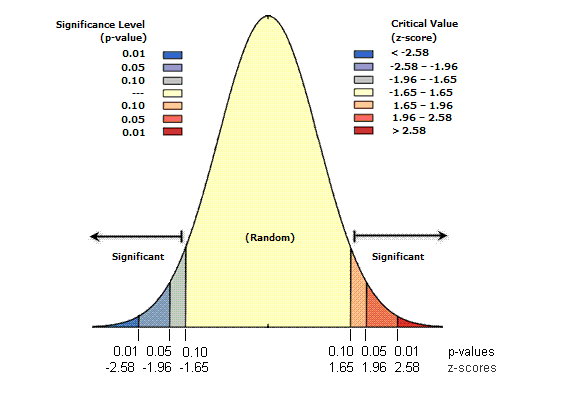
\includegraphics{homework4_answer_key_files/mediabag/z-scores.png}

Calculate \(\alpha\) in the code chunk below for a 95\% confidence
interval.

\begin{Shaded}
\begin{Highlighting}[]
\NormalTok{alpha }\OtherTok{\textless{}{-}} \DecValTok{1} \SpecialCharTok{{-}} \FloatTok{0.95}
\end{Highlighting}
\end{Shaded}

Use the \texttt{qnorm()} function to find the \(Z\)-score which
corresponds to the probability \(\alpha/2\) or \(1-\alpha/2\). Save this
value as \texttt{z\_star}.

\begin{Shaded}
\begin{Highlighting}[]
\NormalTok{z\_star }\OtherTok{\textless{}{-}} \FunctionTok{qnorm}\NormalTok{(alpha}\SpecialCharTok{/}\DecValTok{2}\NormalTok{)}

\NormalTok{z\_star}
\end{Highlighting}
\end{Shaded}

\begin{verbatim}
[1] -1.959964
\end{verbatim}

\begin{Shaded}
\begin{Highlighting}[]
\NormalTok{z\_star }\OtherTok{\textless{}{-}} \FunctionTok{qnorm}\NormalTok{(}\DecValTok{1}\SpecialCharTok{{-}}\NormalTok{alpha}\SpecialCharTok{/}\DecValTok{2}\NormalTok{)}

\NormalTok{z\_star}
\end{Highlighting}
\end{Shaded}

\begin{verbatim}
[1] 1.959964
\end{verbatim}

\subsubsection{Confidence Interval}\label{confidence-interval}

A confidence interval for a single proportion using the
\(Z\)-distribution is calculated as
\(\text{point estimate} \pm Z^* \times SE\).

\paragraph{Trump}\label{trump}

Use the code chunk below to calculate the lower boundary of the 95\%
confidence interval for average proportion of flights delayed during the
Trump administration.

\begin{Shaded}
\begin{Highlighting}[]
\NormalTok{phat\_trump }\SpecialCharTok{{-}}\NormalTok{ z\_star }\SpecialCharTok{*}\NormalTok{ se\_phat\_trump}
\end{Highlighting}
\end{Shaded}

\begin{verbatim}
[1] 0.1326138
\end{verbatim}

Use the code chunk below to calculate the upper boundary of the 95\%
confidence interval for average number of flights delayed during the
Trump administration.

\begin{Shaded}
\begin{Highlighting}[]
\NormalTok{phat\_trump }\SpecialCharTok{+}\NormalTok{ z\_star }\SpecialCharTok{*}\NormalTok{ se\_phat\_trump}
\end{Highlighting}
\end{Shaded}

\begin{verbatim}
[1] 0.205828
\end{verbatim}

Interpret this confidence interval using a complete sentence.

\begin{tcolorbox}[enhanced jigsaw, toprule=.15mm, breakable, leftrule=.75mm, bottomrule=.15mm, rightrule=.15mm, colback=white, opacityback=0, colframe=quarto-callout-warning-color-frame, left=2mm, arc=.35mm]

\textbf{With 95\% confidence, 13.26\% to 20.58\% of flights were delayed
at airports during the Trump administration.}

\end{tcolorbox}

\paragraph{Biden}\label{biden}

Use the code chunk below to calculate the lower boundary of the 95\%
confidence interval for average proportion of flights delayed during the
Biden administration.

\begin{Shaded}
\begin{Highlighting}[]
\NormalTok{phat\_biden }\SpecialCharTok{{-}}\NormalTok{ z\_star }\SpecialCharTok{*}\NormalTok{ se\_phat\_biden}
\end{Highlighting}
\end{Shaded}

\begin{verbatim}
[1] 0.1433887
\end{verbatim}

Use the code chunk below to calculate the upper boundary of the 95\%
confidence interval for average number of flights delayed during the
Biden administration.

\begin{Shaded}
\begin{Highlighting}[]
\NormalTok{phat\_biden }\SpecialCharTok{+}\NormalTok{ z\_star }\SpecialCharTok{*}\NormalTok{ se\_phat\_biden}
\end{Highlighting}
\end{Shaded}

\begin{verbatim}
[1] 0.2191819
\end{verbatim}

Interpret this confidence interval using a complete sentence.

\begin{tcolorbox}[enhanced jigsaw, toprule=.15mm, breakable, leftrule=.75mm, bottomrule=.15mm, rightrule=.15mm, colback=white, opacityback=0, colframe=quarto-callout-warning-color-frame, left=2mm, arc=.35mm]

\textbf{With 95\% confidence, 14.34\% to 21.92\% of flights were delayed
at airports during the Trump administration.}

\end{tcolorbox}

\subsection{Hypothesis Test}\label{hypothesis-test}

Now, you need to test the hypothesis that there's a difference between
the two proportions. Testing for the difference between 2 proportions is
called a \emph{2-sample proportion test}.

Please do a 2-sided hypothesis test with a significance level of
\(\alpha=0.05\).

\begin{enumerate}
\def\labelenumi{\arabic{enumi}.}
\item
  Define your null (\(H_0\)) and alternate (\(H_A\)) hypotheses
  regarding the difference between the 2 proportions
  \(\hat{p}_{\text{Biden}}-\hat{p}_{\text{Trump}}\).
\item
  Calculate a point estimate for the difference between the 2
  proportions \(\hat{p}_{\text{Biden}}-\hat{p}_{\text{Trump}}\) from
  your sample.
\item
  Calculate the standard error \(\operatorname{SE}\) for the difference
  between 2 proportions and infer the sampling distribution of the
  \(\hat{p}_{\text{Biden}}-\hat{p}_{\text{Trump}}\) under your null
  hypothesis.
\item
  Construct a confidence interval under the \(Z\) distribution for the
  difference between the 2 proportions
  \(\hat{p}_{\text{Biden}}-\hat{p}_{\text{Trump}}\) for a significance
  threshold of \(\alpha=0.05\).
\item
  Calculate the test statistic for your observed data
  \(\hat{p}_{\text{Biden}}-\hat{p}_{\text{Trump}}\) under your null
  hypothesis.
\item
  Find the p-value, or the probability of observing a difference between
  proportions \(\hat{p}_{\text{Biden}}-\hat{p}_{\text{Trump}}\) as
  extreme or more extreme than the one you found under the null
  hypothesis.
\item
  Compare your p-value to your significance level \(\alpha\) and choose
  whether or not to reject your null hypothesis \(H_0\).
\end{enumerate}

\subsubsection{Hypothesis Statements}\label{hypothesis-statements}

\paragraph{\texorpdfstring{\(H_0\)}{H\_0}}\label{h_0}

\emph{State your null hypothesis below in 1 sentence.}

\begin{tcolorbox}[enhanced jigsaw, toprule=.15mm, breakable, leftrule=.75mm, bottomrule=.15mm, rightrule=.15mm, colback=white, opacityback=0, colframe=quarto-callout-warning-color-frame, left=2mm, arc=.35mm]

\textbf{Here, you needed to return to the research question motivating
your research.}

\begin{quote}
\emph{Research Question: On average, how frequently were flights delayed
during 2016-2020 and 2021-2024, and were the rates different between the
2 administrations?}
\end{quote}

\textbf{The null hypothesis is a statement of skepticism regarding your
research question. If your research question has you investigating
whether or not there IS a difference, then your null hypothesis should
be that there is NOT a difference.}

\textbf{The null hypothesis is that the difference between the
proportion of flights delayed at airports during the Trump
administration and the proportion of flights delayed at airports during
the Biden administration is 0.}

\(H_0 \colon p_{\text{Biden}}-p_{\text{Trump}}=0\)

\end{tcolorbox}

\paragraph{\texorpdfstring{\(H_A\)}{H\_A}}\label{h_a}

\emph{State your alternative hypothesis below in 1 sentence.}

\begin{tcolorbox}[enhanced jigsaw, toprule=.15mm, breakable, leftrule=.75mm, bottomrule=.15mm, rightrule=.15mm, colback=white, opacityback=0, colframe=quarto-callout-warning-color-frame, left=2mm, arc=.35mm]

\textbf{The alternate hypothesis is a statement regarding the scenario
proposed by your research question. If your research question has you
investigating whether or not there IS a difference, then your alternate
hypothesis should be that there IS a difference.}

\textbf{Additionally, you were asked to do a 2-sided hypothesis test,
which means you do not assume in advance the direction of the
difference. We don't know whether airports under Biden or Trump were
expected to have more delays, so we allow for the possibility of both by
saying that the difference is not 0. If we were doing a 1-sided
hypothesis test, assuming in advance that airports had more delayed
flights under one or the other, we would say that the difference is
greater or less than zero.}

\textbf{The alternate hypothesis is that the difference between the
proportion of flights delayed at airports during the Trump
administration and the proportion of flights delayed at airports during
the Biden administration is not 0.}

\(H_A \colon p_{\text{Biden}}-p_{\text{Trump}} \ne 0\)

\end{tcolorbox}

\subsubsection{Point Estimate}\label{point-estimate}

In the code chunk below, use your variables \texttt{phat\_biden} and
\texttt{phat\_trump} to find
\(\hat{p}_{\text{Biden}}-\hat{p}_{\text{Trump}}\). Save the result as
the variable \texttt{phat\_diff}.

\begin{Shaded}
\begin{Highlighting}[]
\NormalTok{phat\_diff }\OtherTok{\textless{}{-}}\NormalTok{ phat\_biden }\SpecialCharTok{{-}}\NormalTok{ phat\_trump}
\end{Highlighting}
\end{Shaded}

\subsubsection{Standard Error}\label{standard-error}

Use the formula for the standard error of the difference between 2
proportions to calculate
\(\text{SE}_{\hat{p}_{\text{Biden}}-\hat{p}_{\text{Trump}}}\) below and
save it as the variable \texttt{se\_phat\_diff}.

Choose from the formulas below based on your null hypothesis.

\[
\operatorname{SE}_{\text{diff}}=
\begin{cases}
\sqrt{\frac{p_1(1-p_1)}{n_1} + \frac{p_2(1-p_2)}{n_2}}, & \text{when } H_0\colon \hat{p}_1-\hat{p}_2\ne 0 \\
\sqrt{\frac{p_{\text{pool}}(1-p_{\text{pool}})}{n_1} + \frac{p_{\text{pool}}(1-p_{\text{pool}})}{n_2}}, & \text{when } H_0\colon \hat{p}_1-\hat{p}_2 = 0 \\
\end{cases}
\]

\begin{tcolorbox}[enhanced jigsaw, toprule=.15mm, breakable, leftrule=.75mm, bottomrule=.15mm, rightrule=.15mm, colback=white, opacityback=0, colframe=quarto-callout-warning-color-frame, left=2mm, arc=.35mm]

\textbf{Based on your research question, your null hypothesis should
have been} \(H_0: p_1-p_2=0\)\textbf{. You should have chosen the bottom
equation for the standard error of the difference between 2 proportions
and completed the steps below.}

\end{tcolorbox}

If your null hypothesis is \(H_0\colon \hat{p}_1-\hat{p}_2\ne 0\), you
will also need to calculate \(\hat{p}_{\text{pool}}\). That's because
this hypothesis states that the two samples come from the same
population. Therefore, we only need 1 parameter
\(\hat{p}_{\text{pool}}\) for the population.

\[
\hat{p}_{\text{pool}}=\frac{\text{count}(\text{delays})_{\text{Trump}} + \text{count}(\text{delays})_{\text{Biden}}}{\text{count}(\text{flights})_{\text{Trump}} + \text{count}(\text{flights})_{\text{Biden}}}
\]

Use the \texttt{summarize()} function from the \texttt{dplyr} package to
find the sample size (\(n\)), the total number of flights
(\texttt{flights}), and the total number of delayed flights
(\texttt{delayed}), but do not include a \texttt{.by} parameter to
separate the results by administration.

\begin{Shaded}
\begin{Highlighting}[]
\NormalTok{proportion\_statistics2 }\OtherTok{\textless{}{-}}\NormalTok{ delays }\SpecialCharTok{|\textgreater{}}
  \FunctionTok{summarize}\NormalTok{(}\AttributeTok{n =} \FunctionTok{n}\NormalTok{(), }
            \AttributeTok{flights =} \FunctionTok{sum}\NormalTok{(flights), }
            \AttributeTok{delayed =} \FunctionTok{sum}\NormalTok{(delayed), }
            \AttributeTok{proportion =} \FunctionTok{sum}\NormalTok{(delayed) }\SpecialCharTok{/} \FunctionTok{sum}\NormalTok{(flights))}

\NormalTok{proportion\_statistics2}
\end{Highlighting}
\end{Shaded}

\begin{verbatim}
# A tibble: 1 x 4
      n  flights delayed proportion
  <int>    <dbl>   <dbl>      <dbl>
1   800 56146163 9834362      0.175
\end{verbatim}

If you need to calculate \(\hat{p}_{\text{pool}}\), use the code chunk
below to save the result as the variable \texttt{phat\_pool}.

\begin{Shaded}
\begin{Highlighting}[]
\NormalTok{phat\_pool }\OtherTok{\textless{}{-}} \DecValTok{10001276}\SpecialCharTok{/}\DecValTok{56939821}
\end{Highlighting}
\end{Shaded}

Use the code chunk below to find the standard error of the difference
\(\text{SE}_{\hat{p}_{\text{Biden}}-\hat{p}_{\text{Trump}}}\) under your
null hypothesis. Save the result as \texttt{se\_phat\_diff}.

\begin{Shaded}
\begin{Highlighting}[]
\NormalTok{se\_phat\_diff }\OtherTok{\textless{}{-}} \FunctionTok{sqrt}\NormalTok{((phat\_pool}\SpecialCharTok{*}\NormalTok{(}\DecValTok{1}\SpecialCharTok{{-}}\NormalTok{phat\_pool))}\SpecialCharTok{/}\NormalTok{n\_trump }\SpecialCharTok{+}\NormalTok{ (phat\_pool}\SpecialCharTok{*}\NormalTok{(}\DecValTok{1}\SpecialCharTok{{-}}\NormalTok{phat\_pool))}\SpecialCharTok{/}\NormalTok{n\_biden)}

\NormalTok{se\_phat\_diff}
\end{Highlighting}
\end{Shaded}

\begin{verbatim}
[1] 0.02690752
\end{verbatim}

\subsubsection{Critical Score}\label{critical-score}

The difference of 2 proportions uses the \(Z\) distribution, so the
critical score for this confidence interval is \(Z^*\). Find the
\(Z\)-score for the probability \(\alpha/2\) or \(1-\alpha/2\) using the
\texttt{qnorm()} function.

\begin{Shaded}
\begin{Highlighting}[]
\NormalTok{z\_star }\OtherTok{\textless{}{-}} \FunctionTok{qnorm}\NormalTok{(alpha}\SpecialCharTok{/}\DecValTok{2}\NormalTok{)}

\NormalTok{z\_star}
\end{Highlighting}
\end{Shaded}

\begin{verbatim}
[1] -1.959964
\end{verbatim}

\begin{Shaded}
\begin{Highlighting}[]
\NormalTok{z\_star }\OtherTok{\textless{}{-}} \FunctionTok{qnorm}\NormalTok{(}\DecValTok{1}\SpecialCharTok{{-}}\NormalTok{alpha}\SpecialCharTok{/}\DecValTok{2}\NormalTok{)}

\NormalTok{z\_star}
\end{Highlighting}
\end{Shaded}

\begin{verbatim}
[1] 1.959964
\end{verbatim}

\subsubsection{Confidence Interval}\label{confidence-interval-1}

As with the 1-sample proportions, the confidence interval for the
difference between 2 proportions is calculated as
\(\text{point estimate} \pm Z^* \times SE\).

Use the code chunk below to calculate the lower boundary of your
confidence interval for average difference in the proportion of flights
delayed during the Trump administration and proportion of flights
delayed during the Biden administration.

\begin{Shaded}
\begin{Highlighting}[]
\NormalTok{phat\_diff }\SpecialCharTok{{-}}\NormalTok{ z\_star }\SpecialCharTok{*}\NormalTok{ se\_phat\_diff}
\end{Highlighting}
\end{Shaded}

\begin{verbatim}
[1] -0.04067336
\end{verbatim}

Use the code chunk below to calculate the upper boundary of your
confidence interval for average difference in the proportion of flights
delayed during the Trump administration and proportion of flights
delayed during the Biden administration.

\begin{Shaded}
\begin{Highlighting}[]
\NormalTok{phat\_diff }\SpecialCharTok{+}\NormalTok{ z\_star }\SpecialCharTok{*}\NormalTok{ se\_phat\_diff}
\end{Highlighting}
\end{Shaded}

\begin{verbatim}
[1] 0.06480217
\end{verbatim}

Interpret this confidence interval in 1 sentence.

\begin{tcolorbox}[enhanced jigsaw, toprule=.15mm, breakable, leftrule=.75mm, bottomrule=.15mm, rightrule=.15mm, colback=white, opacityback=0, colframe=quarto-callout-warning-color-frame, left=2mm, arc=.35mm]

\textbf{With 95\% confidence, the difference between the proportion of
flights delayed more than 15 minutes at airports during the Biden
administration and the proportion of flights delayed more than 15
minutes at airports during the Trump administration was -4.1\% to
6.5\%.}

\end{tcolorbox}

\subsubsection{Test Statistic}\label{test-statistic}

Calculate the test statistic \(Z\) under your null distribution for your
observed value
\(\text{SE}_{\hat{p}_{\text{Biden}}-\hat{p}_{\text{Trump}}}\). Save the
value as \texttt{z\_diff}.

\[
Z=
\begin{cases}
\frac{(\hat{p}_1-\hat{p}_2)-\mu}{\text{SE}}, & \text{when } H_0\colon \hat{p}_1-\hat{p}_2 \ne 0 \\
\frac{\hat{p}_1-\hat{p}_2}{\text{SE}}, & \text{when } H_0\colon \hat{p}_1-\hat{p}_2 = 0
\end{cases}
\]

\begin{tcolorbox}[enhanced jigsaw, toprule=.15mm, breakable, leftrule=.75mm, bottomrule=.15mm, rightrule=.15mm, colback=white, opacityback=0, colframe=quarto-callout-warning-color-frame, left=2mm, arc=.35mm]

\textbf{Based on your research question, your null hypothesis should
have been} \(H_0: p_1-p_2=0\)\textbf{. You should have chosen the bottom
equation for the test statistic calculation.}

\end{tcolorbox}

\begin{Shaded}
\begin{Highlighting}[]
\NormalTok{z\_diff }\OtherTok{\textless{}{-}}\NormalTok{ phat\_diff}\SpecialCharTok{/}\NormalTok{se\_phat\_diff}

\NormalTok{z\_diff}
\end{Highlighting}
\end{Shaded}

\begin{verbatim}
[1] 0.4483655
\end{verbatim}

Interpret the test statistic in 1 sentence.

\begin{tcolorbox}[enhanced jigsaw, toprule=.15mm, breakable, leftrule=.75mm, bottomrule=.15mm, rightrule=.15mm, colback=white, opacityback=0, colframe=quarto-callout-warning-color-frame, left=2mm, arc=.35mm]

\textbf{In our sample, we observed that 1.2\% more flights were delayed
more than 15 minutes at airports during the Biden administration than
during the Trump administration, which is 0.45 standard errors above the
null hypothesis that there was no difference in the proportion of
flights delayed more than 15 minutes at airports during the two
administrations.}

\end{tcolorbox}

\subsubsection{P-Value}\label{p-value}

Find the p-value for your test statistic \texttt{z\_diff} using the
function \texttt{pnorm()}. Use a 2-sided hypothesis test.

\begin{Shaded}
\begin{Highlighting}[]
\FunctionTok{pnorm}\NormalTok{(z\_diff, }\AttributeTok{lower.tail =}\NormalTok{ F) }\SpecialCharTok{*} \DecValTok{2}
\end{Highlighting}
\end{Shaded}

\begin{verbatim}
[1] 0.6538894
\end{verbatim}

\subsubsection{Decision}\label{decision}

Given the p-value for your observed data under the null hypothesis and a
significance threshold of \(\alpha=0.05\), would you reject the null
hypothesis? Why or why not?

\begin{tcolorbox}[enhanced jigsaw, toprule=.15mm, breakable, leftrule=.75mm, bottomrule=.15mm, rightrule=.15mm, colback=white, opacityback=0, colframe=quarto-callout-warning-color-frame, left=2mm, arc=.35mm]

\textbf{The p-value of 0.654 is greater than our significance threshold
of 0.05, so you should not have rejected the null hypothesis with this
data.}

\textbf{If the null hypothesis were true, the difference between the
proportion of flights delayed at airports during the Trump and Biden
administrations is 0. Assuming the null hypothesis is true, the
probability of taking two samples of size} \(n_{\text{Trump}}=403\)
\textbf{and} \(n_{\text{Biden}}=397\) \textbf{from this study population
and seeing a probability difference more extreme than the one we got in
our sample (greater than 1.2\% or less than -1.2\%) is 65\%.}

\textbf{In other words, if there were no real difference and you
repeated this study over and over, you would get}
\(\hat{p}_{\text{Biden}}-\hat{p}_{\text{Trump}}>0.012\) \textbf{or}
\(\hat{p}_{\text{Biden}}-\hat{p}_{\text{Trump}}<-0.012\) \textbf{about
65\% of the time. To reject a null hypothesis, we need our observed data
to be UNLIKELY under the null hypothesis, or a small p-value. When the
observed data is unlikely under the null hypothesis, we can reject that
theory of the world and accept the alternate hypothesis. Here, however,
our data is consistent with the null hypothesis, so we fail to reject
it.}

\textbf{This study did not detect a difference between the proportion of
flights delayed more than 15 minutes at airports during the Trump and
Biden administrations.}

\end{tcolorbox}

\section{Means}\label{means}

\textbf{\emph{Research Question: On average, how many minutes were
flights delayed during 2016-2020 and 2021-2024, and were the times
different between the 2 administrations?}}

\begin{enumerate}
\def\labelenumi{\arabic{enumi}.}
\item
  Calculate your sample statistics from your data: the length of delays
  during the Trump (\(\bar{x}_{\text{Trump}}\)) and Biden
  administrations (\(\bar{x}_{\text{Biden}}\)).
\item
  Check the sample size assumption.
\item
  Infer the average delay length in the US during the Trump and Biden
  administrations from your sample statistics.
\item
  Test the hypothesis that the average delay during the Trump
  administration is different from the average delay during the Biden
  administration.
\end{enumerate}

\subsection{Sample Statistics}\label{sample-statistics-1}

Use the \texttt{summarize()} function from the \texttt{dplyr} package to
find the sample size (\(n\)), the mean (\texttt{mean}) of the average
delay times in minutes (\texttt{avg\_delay}), and standard deviation
(\texttt{sd}) of the average delay times in minutes.

\begin{Shaded}
\begin{Highlighting}[]
\NormalTok{mean\_statistics }\OtherTok{\textless{}{-}}\NormalTok{ delays }\SpecialCharTok{|\textgreater{}}
  \FunctionTok{summarize}\NormalTok{(}\AttributeTok{n =} \FunctionTok{n}\NormalTok{(), }
            \AttributeTok{mean =} \FunctionTok{mean}\NormalTok{(avg\_delay), }
            \AttributeTok{sd =} \FunctionTok{sd}\NormalTok{(avg\_delay),}
            \AttributeTok{.by =} \StringTok{\textquotesingle{}admin\textquotesingle{}}\NormalTok{)}

\NormalTok{mean\_statistics }
\end{Highlighting}
\end{Shaded}

\begin{verbatim}
# A tibble: 2 x 4
  admin     n  mean    sd
  <chr> <int> <dbl> <dbl>
1 Trump   397  11.3  4.69
2 Biden   403  12.6 11.1 
\end{verbatim}

Save your point estimate of \(\bar{x}_{\text{Trump}}\) rounded to 2
decimal places as the variable \texttt{mean\_trump}.

\begin{Shaded}
\begin{Highlighting}[]
\NormalTok{mean\_trump }\OtherTok{\textless{}{-}} \FloatTok{11.27}

\NormalTok{mean\_trump}
\end{Highlighting}
\end{Shaded}

\begin{verbatim}
[1] 11.27
\end{verbatim}

Save your point estimate of \(\bar{x}_{\text{Biden}}\) rounded to 2
decimal places as the variable \texttt{mean\_biden}.

\begin{Shaded}
\begin{Highlighting}[]
\NormalTok{mean\_biden }\OtherTok{\textless{}{-}} \FloatTok{12.56}

\NormalTok{mean\_biden}
\end{Highlighting}
\end{Shaded}

\begin{verbatim}
[1] 12.56
\end{verbatim}

Save your point estimate of \(s_{\text{Trump}}\) rounded to 2 decimal
places as the variable \texttt{sd\_trump}.

\begin{Shaded}
\begin{Highlighting}[]
\NormalTok{sd\_trump }\OtherTok{\textless{}{-}} \FloatTok{4.69}

\NormalTok{sd\_trump}
\end{Highlighting}
\end{Shaded}

\begin{verbatim}
[1] 4.69
\end{verbatim}

Save your point estimate of \(s_{\text{Biden}}\) rounded to 2 decimal
places as the variable \texttt{sd\_biden}.

\begin{Shaded}
\begin{Highlighting}[]
\NormalTok{sd\_biden }\OtherTok{\textless{}{-}} \FloatTok{11.09}

\NormalTok{sd\_biden}
\end{Highlighting}
\end{Shaded}

\begin{verbatim}
[1] 11.09
\end{verbatim}

\subsection{Assumptions}\label{assumptions-1}

For the Central Limit Theorem to apply for means, there must be at least
\(n\ge30\) observations.

In the code chunk below, check the assumption that you have at least 30
observations from the Trump administration.

\begin{Shaded}
\begin{Highlighting}[]
\NormalTok{n\_trump}
\end{Highlighting}
\end{Shaded}

\begin{verbatim}
[1] 403
\end{verbatim}

\begin{tcolorbox}[enhanced jigsaw, toprule=.15mm, breakable, leftrule=.75mm, bottomrule=.15mm, rightrule=.15mm, colback=white, opacityback=0, colframe=quarto-callout-warning-color-frame, left=2mm, arc=.35mm]

\textbf{The sample statistic} \(\bar{x}_{\text{Trump}}\) \textbf{is
based on data from 403 airports under the Trump administration, which is
more than 30.}

\end{tcolorbox}

In the code chunk below, check the assumption that you have at least 30
observations from the Biden administration.

\begin{Shaded}
\begin{Highlighting}[]
\NormalTok{n\_biden}
\end{Highlighting}
\end{Shaded}

\begin{verbatim}
[1] 397
\end{verbatim}

\begin{tcolorbox}[enhanced jigsaw, toprule=.15mm, breakable, leftrule=.75mm, bottomrule=.15mm, rightrule=.15mm, colback=white, opacityback=0, colframe=quarto-callout-warning-color-frame, left=2mm, arc=.35mm]

\textbf{The sample statistic} \(\bar{x}_{\text{Biden}}\) \textbf{is
based on data from 397 airports under the Trump administration, which is
more than 30.}

\end{tcolorbox}

\subsection{Inference}\label{inference-1}

Once you have checked your assumptions, you can use the Central Limit
Theorem to infer the sampling distribution of \(\bar{x}\) in the study
population.

The Central Limit Theorem states that as the sample size \(n\) increases
(\(n \to \infty\)), the distribution of the sample statistic \(\bar{x}\)
approximates a normal distribution with mean \(\mu\) and standard
deviation \(\operatorname{SE}\) or the standard error of a mean

\[
\begin{aligned}
\bar{x} &\sim \operatorname{N}\left(\mu, \operatorname{SE}\right)
\end{aligned}
\]

The standard deviation for this sampling distribution, the standard
error \(\operatorname{SE}\) of a single sample mean \(\bar{x}\), is
calculated as follows.

\[
\operatorname{SE}=\frac{\sigma}{\sqrt{n}}
\]

However, the population parameter \(s\), the ``true'' standard
deviation, is ``unknowable'' unless you have all the data possible. You
have a random sample, so you can not directly observed \(\sigma\).

However, when the data in your sample is valid, \(\bar{x} \approx \mu\)
and can be used to infer the sampling distribution of \(\bar{x}\). We
also use \(s\) as an estimate for \(\sigma\), but we will need to
account for the additional uncertainty of using 2 estimated statistics
in our distribution.

\[
\begin{aligned}
\bar{x} &\sim \operatorname{N}\left(\bar{x}, \frac{s}{\sqrt{n}}\right)
\end{aligned}
\]

Work through the steps below to infer the sampling distributions for
\(\bar{x}_{\text{Trump}}\) and \(\bar{x}_{\text{Biden}}\) as
\(\bar{x} \sim \operatorname{N}\left(\bar{x}, \operatorname{SE}\right)\).

You calculated your point estimates for \(\bar{x}_{\text{Trump}}\) and
\(\bar{x}_{\text{Biden}}\) in the last section. Now, you will calculate
the standard errors \(\operatorname{SE}_{\text{Trump}}\) and
\(\operatorname{SE}_{\text{Biden}}\).

Use these sampling distributions to calculate 95\% confidence intervals
for the average delay during each administration.

Because we do not know \(\sigma\) and are approximating it with the
sample statistic \(s\), we need to account for the additional
uncertainty in our estimates. We use the \(T\) or Student's \(t\)
distribution for inference when we don't know \(\sigma\).

\[
\text{point estimate} \pm T^*_{\text{df}} \times SE
\]

The critical value \(T^*\) corresponds to the \(T\)-score for the
probability \(\alpha/2\) or \(1-\alpha/2\). You can find \(\alpha\) from
the confidence level. The \(T\)-distribution has an additional parameter
called degrees of freedom..

\[
\text{df}=n-1
\]

\subsubsection{Standard Errors}\label{standard-errors-1}

Use the formula for the standard error of a single mean to calculate
\(\operatorname{SE}_{\text{Trump}}\) below and save it as the variable
\texttt{se\_mean\_trump}.

\begin{Shaded}
\begin{Highlighting}[]
\NormalTok{se\_mean\_trump }\OtherTok{\textless{}{-}}\NormalTok{ sd\_trump }\SpecialCharTok{/} \FunctionTok{sqrt}\NormalTok{(n\_trump)}

\NormalTok{se\_mean\_trump}
\end{Highlighting}
\end{Shaded}

\begin{verbatim}
[1] 0.2336255
\end{verbatim}

Use the formula for the standard error of a single proportion to
calculate \(\operatorname{SE}_{\text{Biden}}\) below and save it as the
variable \texttt{se\_mean\_biden}.

\begin{Shaded}
\begin{Highlighting}[]
\NormalTok{se\_mean\_biden }\OtherTok{\textless{}{-}}\NormalTok{ sd\_biden }\SpecialCharTok{/} \FunctionTok{sqrt}\NormalTok{(n\_biden)}

\NormalTok{se\_mean\_biden}
\end{Highlighting}
\end{Shaded}

\begin{verbatim}
[1] 0.5565911
\end{verbatim}

\subsubsection{Critical Value}\label{critical-value-1}

The \emph{critical value} \(T^*\) for a 95\% confidence interval from
the \(T\) distribution indicates how many standard errors away from the
mean delay (\(\mu\)) that 95\% of the data can be in this distribution.
In other words, 95\% of the data in this distribution falls between
\(-T^*\) and \(T^*\).

Calculate \(\alpha\) in the code chunk below for a 95\% confidence
interval.

\begin{Shaded}
\begin{Highlighting}[]
\NormalTok{alpha }\OtherTok{\textless{}{-}} \DecValTok{1} \SpecialCharTok{{-}} \FloatTok{0.95}
\end{Highlighting}
\end{Shaded}

Use the \texttt{qt()} function to find the \(T\)-score which corresponds
to the probability \(\alpha/2\) or \(1-\alpha/2\) for the Trump
administration. The \texttt{qt()} function takes the additional
parameter \(\text{df}=n-1\). Save this value as \texttt{t\_star\_trump}.

\begin{Shaded}
\begin{Highlighting}[]
\NormalTok{t\_star\_trump }\OtherTok{\textless{}{-}} \FunctionTok{qt}\NormalTok{(alpha}\SpecialCharTok{/}\DecValTok{2}\NormalTok{, }
                   \AttributeTok{df =}\NormalTok{ n\_trump}\DecValTok{{-}1}\NormalTok{)}

\NormalTok{t\_star\_trump}
\end{Highlighting}
\end{Shaded}

\begin{verbatim}
[1] -1.965883
\end{verbatim}

\begin{Shaded}
\begin{Highlighting}[]
\NormalTok{t\_star\_trump }\OtherTok{\textless{}{-}} \FunctionTok{qt}\NormalTok{(}\DecValTok{1}\SpecialCharTok{{-}}\NormalTok{alpha}\SpecialCharTok{/}\DecValTok{2}\NormalTok{, }
                   \AttributeTok{df =}\NormalTok{ n\_trump}\DecValTok{{-}1}\NormalTok{)}

\NormalTok{t\_star\_trump}
\end{Highlighting}
\end{Shaded}

\begin{verbatim}
[1] 1.965883
\end{verbatim}

Use the \texttt{qt()} function to find the \(T\)-score which corresponds
to the probability \(\alpha/2\) or \(1-\alpha/2\) for the Biden
administration. Save this value as \texttt{t\_star\_biden}.

\begin{Shaded}
\begin{Highlighting}[]
\NormalTok{t\_star\_biden }\OtherTok{\textless{}{-}} \FunctionTok{qt}\NormalTok{(alpha}\SpecialCharTok{/}\DecValTok{2}\NormalTok{, }
                   \AttributeTok{df =}\NormalTok{ n\_biden}\DecValTok{{-}1}\NormalTok{)}

\NormalTok{t\_star\_biden}
\end{Highlighting}
\end{Shaded}

\begin{verbatim}
[1] -1.965973
\end{verbatim}

\begin{Shaded}
\begin{Highlighting}[]
\NormalTok{t\_star\_biden }\OtherTok{\textless{}{-}} \FunctionTok{qt}\NormalTok{(}\DecValTok{1}\SpecialCharTok{{-}}\NormalTok{alpha}\SpecialCharTok{/}\DecValTok{2}\NormalTok{, }
                   \AttributeTok{df =}\NormalTok{ n\_biden}\DecValTok{{-}1}\NormalTok{)}

\NormalTok{t\_star\_biden}
\end{Highlighting}
\end{Shaded}

\begin{verbatim}
[1] 1.965973
\end{verbatim}

Compare your \(T^*\)'s to your \(Z^*\) from your proportions. Comment in
1 sentence on why they are similar or different.

\begin{tcolorbox}[enhanced jigsaw, toprule=.15mm, breakable, leftrule=.75mm, bottomrule=.15mm, rightrule=.15mm, colback=white, opacityback=0, colframe=quarto-callout-warning-color-frame, left=2mm, arc=.35mm]

\textbf{The values from the Z distribution are smaller because it is a
narrower distribution. 95\% of the data is closer to the mean of the
distribution, so the critical values will be closer to 0. The T
distribution is wider to account for the uncertainty of using an
estimated standard deviation to calculate the standard error. Therefore,
you need to be further from 0 to capture 95\% of the data.}

\end{tcolorbox}

\subsubsection{Confidence Interval}\label{confidence-interval-2}

A confidence interval for a single mean using the \(T\)-distribution
with degrees of freedom \(n-1\) is calculated as
\(\text{point estimate} \pm T^*_{\text{df}} \times SE\).

\paragraph{Trump}\label{trump-1}

Use the code chunk below to calculate the lower boundary of the 95\%
confidence interval for average delay during the Trump administration.

\begin{Shaded}
\begin{Highlighting}[]
\NormalTok{mean\_trump }\SpecialCharTok{{-}}\NormalTok{ t\_star\_trump }\SpecialCharTok{*}\NormalTok{ se\_mean\_trump}
\end{Highlighting}
\end{Shaded}

\begin{verbatim}
[1] 10.81072
\end{verbatim}

Use the code chunk below to calculate the upper boundary of the 95\%
confidence interval for average delay during the Trump administration.

\begin{Shaded}
\begin{Highlighting}[]
\NormalTok{mean\_trump }\SpecialCharTok{+}\NormalTok{ t\_star\_trump }\SpecialCharTok{*}\NormalTok{ se\_mean\_trump}
\end{Highlighting}
\end{Shaded}

\begin{verbatim}
[1] 11.72928
\end{verbatim}

Interpret this confidence interval using a complete sentence.

\begin{tcolorbox}[enhanced jigsaw, toprule=.15mm, breakable, leftrule=.75mm, bottomrule=.15mm, rightrule=.15mm, colback=white, opacityback=0, colframe=quarto-callout-warning-color-frame, left=2mm, arc=.35mm]

\textbf{With 95\% confidence, flights were delayed 10.81-11.73 minutes
on average at airports during the Trump administration.}

\end{tcolorbox}

\paragraph{Biden}\label{biden-1}

Use the code chunk below to calculate the lower boundary of the 95\%
confidence interval for average delay during the Biden administration.

\begin{Shaded}
\begin{Highlighting}[]
\NormalTok{mean\_biden }\SpecialCharTok{{-}}\NormalTok{ t\_star\_biden }\SpecialCharTok{*}\NormalTok{ se\_mean\_biden}
\end{Highlighting}
\end{Shaded}

\begin{verbatim}
[1] 11.46576
\end{verbatim}

Use the code chunk below to calculate the upper boundary of the 95\%
confidence interval for average delay during the Biden administration.

\begin{Shaded}
\begin{Highlighting}[]
\NormalTok{mean\_biden }\SpecialCharTok{+}\NormalTok{ t\_star\_biden }\SpecialCharTok{*}\NormalTok{ se\_mean\_biden}
\end{Highlighting}
\end{Shaded}

\begin{verbatim}
[1] 13.65424
\end{verbatim}

Interpret this confidence interval using a complete sentence.

\begin{tcolorbox}[enhanced jigsaw, toprule=.15mm, breakable, leftrule=.75mm, bottomrule=.15mm, rightrule=.15mm, colback=white, opacityback=0, colframe=quarto-callout-warning-color-frame, left=2mm, arc=.35mm]

\textbf{With 95\% confidence, flights were delayed 11.47-13.65 minutes
on average at airports during the Biden administration.}

\end{tcolorbox}

\subsection{Hypothesis Test}\label{hypothesis-test-1}

Now, you need to test the hypothesis that there's a difference between
the two means. Testing for the difference between 2 proportions is
called a \emph{2-sample} \(t\) test.

Please do a 2-sided hypothesis test with a significance level of
\(\alpha=0.05\).

\begin{enumerate}
\def\labelenumi{\arabic{enumi}.}
\item
  Define your null (\(H_0\)) and alternate (\(H_A\)) hypotheses
  regarding the difference between the 2 proportions
  \(\bar{x}_{\text{Biden}}-\bar{x}_{\text{Trump}}\).
\item
  Calculate a point estimate for the difference between the 2
  proportions \(\bar{x}_{\text{Biden}}-\bar{x}_{\text{Trump}}\) from
  your sample.
\item
  Calculate the standard error \(\operatorname{SE}\) for the difference
  between 2 proportions and infer the sampling distribution of the
  \(\bar{x}_{\text{Biden}}-\bar{x}_{\text{Trump}}\) under your null
  hypothesis.
\item
  Construct a confidence interval under the \(T\) distribution for the
  difference between the 2 proportions
  \(\bar{x}_{\text{Biden}}-\bar{x}_{\text{Trump}}\) for a significance
  threshold of \(\alpha=0.05\).
\item
  Calculate the test statistic for your observed data
  \(\bar{x}_{\text{Biden}}-\bar{x}_{\text{Trump}}\) under your null
  hypothesis.
\item
  Find the p-value, or the probability of observing a difference between
  means \(\bar{x}_{\text{Biden}}-\bar{x}_{\text{Trump}}\) as extreme or
  more extreme than the one you found under the null hypothesis.
\item
  Compare your p-value to your significance level \(\alpha\) and choose
  whether or not to reject your null hypothesis \(H_0\).
\end{enumerate}

\subsubsection{Hypothesis Statements}\label{hypothesis-statements-1}

\paragraph{\texorpdfstring{\(H_0\)}{H\_0}}\label{h_0-1}

\emph{State your null hypothesis below in 1 sentence.}

\begin{tcolorbox}[enhanced jigsaw, toprule=.15mm, breakable, leftrule=.75mm, bottomrule=.15mm, rightrule=.15mm, colback=white, opacityback=0, colframe=quarto-callout-warning-color-frame, left=2mm, arc=.35mm]

\textbf{Here, you needed to return to the research question motivating
your research.}

\begin{quote}
\emph{Research Question: On average, how many minutes were flights
delayed during 2016-2020 and 2021-2024, and were the times different
between the 2 administrations?}
\end{quote}

\textbf{The null hypothesis is a statement of skepticism regarding your
research question. If your research question has you investigating
whether or not there IS a difference, then your null hypothesis should
be that there is NOT a difference.}

\textbf{The null hypothesis is that the difference between the average
delay time at airports during the Trump administration and the average
delay time at airports during the Biden administration is 0.}

\(H_0 \colon \mu_{\text{Biden}}-\mu_{\text{Trump}}=0\)

\end{tcolorbox}

\paragraph{\texorpdfstring{\(H_A\)}{H\_A}}\label{h_a-1}

\emph{State your alternative hypothesis below in 1 sentence.}

\begin{tcolorbox}[enhanced jigsaw, toprule=.15mm, breakable, leftrule=.75mm, bottomrule=.15mm, rightrule=.15mm, colback=white, opacityback=0, colframe=quarto-callout-warning-color-frame, left=2mm, arc=.35mm]

\textbf{The alternate hypothesis is a statement regarding the scenario
proposed by your research question. If your research question has you
investigating whether or not there IS a difference, then your alternate
hypothesis should be that there IS a difference.}

\textbf{Additionally, you were asked to do a 2-sided hypothesis test,
which means you do not assume in advance the direction of the
difference. We don't know whether airports under Biden or Trump were
expected to have longer delays, so we allow for the possibility of both
by saying that the difference is not 0. If we were doing a 1-sided
hypothesis test, assuming in advance that airports had longer delays
under one or the other, we would say that the difference is greater or
less than zero.}

\textbf{The alternate hypothesis is that the difference between the
average delay time at airports during the Trump administration and the
average delay time at airports during the Biden administration is not
0.}

\(H_A \colon \mu_{\text{Biden}}-\mu_{\text{Trump}} \ne 0\)

\end{tcolorbox}

\subsubsection{Point Estimate}\label{point-estimate-1}

In the code chunk below, use your variables \texttt{mean\_biden} and
\texttt{mean\_trump} to find
\(\bar{x}_{\text{Biden}}-\bar{x}_{\text{Trump}}\). Save the result as
the variable \texttt{mean\_diff}.

\begin{Shaded}
\begin{Highlighting}[]
\NormalTok{mean\_diff }\OtherTok{\textless{}{-}}\NormalTok{ mean\_biden }\SpecialCharTok{{-}}\NormalTok{ mean\_trump}

\NormalTok{mean\_diff}
\end{Highlighting}
\end{Shaded}

\begin{verbatim}
[1] 1.29
\end{verbatim}

\subsubsection{Standard Error}\label{standard-error-1}

Use the formula for the standard error of the difference between 2
proportions to calculate
\(\text{SE}_{\bar{x}_{\text{Biden}}-\bar{x}_{\text{Trump}}}\) below and
save it as the variable \texttt{se\_mean\_diff}.

\[
\text{SE}=\sqrt{\frac{s_1^2}{n_1}+\frac{s_2^2}{n_2}}
\]

Use the code chunk below to find the standard error of the difference
\(\text{SE}_{\bar{x}_{\text{Biden}}-\bar{x}_{\text{Trump}}}\) under your
null hypothesis. Save the result as \texttt{se\_mean\_diff}.

\begin{Shaded}
\begin{Highlighting}[]
\NormalTok{se\_mean\_diff }\OtherTok{\textless{}{-}} \FunctionTok{sqrt}\NormalTok{((sd\_trump}\SpecialCharTok{\^{}}\DecValTok{2}\NormalTok{)}\SpecialCharTok{/}\NormalTok{n\_trump }\SpecialCharTok{+}\NormalTok{ (sd\_biden}\SpecialCharTok{\^{}}\DecValTok{2}\NormalTok{)}\SpecialCharTok{/}\NormalTok{n\_biden)}

\NormalTok{se\_mean\_diff}
\end{Highlighting}
\end{Shaded}

\begin{verbatim}
[1] 0.6036345
\end{verbatim}

\subsubsection{Critical Score}\label{critical-score-1}

The difference of 2 means uses the \(T\) distribution with the degrees
of freedom \(\text{df}=min(n_1, n_2)-1\), so the critical score for this
confidence interval is \(T^*_{\text{df}}\).

Use the code chunk below to find the degrees of freedom for the
difference in means using the \texttt{min()} function. Save the result
as \texttt{dof}.

\begin{Shaded}
\begin{Highlighting}[]
\NormalTok{dof }\OtherTok{\textless{}{-}} \FunctionTok{min}\NormalTok{(n\_trump, n\_biden)}\SpecialCharTok{{-}}\DecValTok{1}
\end{Highlighting}
\end{Shaded}

Find the \(T\)-score for the probability \(\alpha/2\) or \(1-\alpha/2\)
using the \texttt{qt()} function and the parameter \texttt{df} set to
the degrees of freedom you just calculated. Save the value as
\texttt{t\_star\_diff}

\begin{Shaded}
\begin{Highlighting}[]
\NormalTok{t\_star\_diff }\OtherTok{\textless{}{-}} \FunctionTok{qt}\NormalTok{(alpha}\SpecialCharTok{/}\DecValTok{2}\NormalTok{, }
                  \AttributeTok{df =}\NormalTok{ dof)}

\NormalTok{t\_star\_diff}
\end{Highlighting}
\end{Shaded}

\begin{verbatim}
[1] -1.965973
\end{verbatim}

\begin{Shaded}
\begin{Highlighting}[]
\NormalTok{t\_star\_diff }\OtherTok{\textless{}{-}} \FunctionTok{qt}\NormalTok{(}\DecValTok{1}\SpecialCharTok{{-}}\NormalTok{alpha}\SpecialCharTok{/}\DecValTok{2}\NormalTok{, }
                  \AttributeTok{df =}\NormalTok{ dof)}

\NormalTok{t\_star\_diff}
\end{Highlighting}
\end{Shaded}

\begin{verbatim}
[1] 1.965973
\end{verbatim}

\subsubsection{Confidence Interval}\label{confidence-interval-3}

As with the 1-sample means, the confidence interval for the difference
between 2 means is calculated as
\(\text{point estimate} \pm T^*_{\text{df}} \times SE\).

Use the code chunk below to calculate the lower boundary of your
confidence interval for average difference in the proportion of flights
delayed during the Trump administration and proportion of flights
delayed during the Biden administration.

\begin{Shaded}
\begin{Highlighting}[]
\NormalTok{mean\_diff }\SpecialCharTok{{-}}\NormalTok{ t\_star\_diff }\SpecialCharTok{*}\NormalTok{ se\_mean\_diff}
\end{Highlighting}
\end{Shaded}

\begin{verbatim}
[1] 0.1032711
\end{verbatim}

Use the code chunk below to calculate the upper boundary of your
confidence interval for average difference in the proportion of flights
delayed during the Trump administration and proportion of flights
delayed during the Biden administration.

\begin{Shaded}
\begin{Highlighting}[]
\NormalTok{mean\_diff }\SpecialCharTok{+}\NormalTok{ t\_star\_diff }\SpecialCharTok{*}\NormalTok{ se\_mean\_diff}
\end{Highlighting}
\end{Shaded}

\begin{verbatim}
[1] 2.476729
\end{verbatim}

Interpret this confidence interval in 1 sentence.

\begin{tcolorbox}[enhanced jigsaw, toprule=.15mm, breakable, leftrule=.75mm, bottomrule=.15mm, rightrule=.15mm, colback=white, opacityback=0, colframe=quarto-callout-warning-color-frame, left=2mm, arc=.35mm]

\textbf{With 95\% confidence, flights were delayed 0.10 to 2.48 minutes
longer at airports during the Biden administration than during the Trump
administration.}

\end{tcolorbox}

\subsubsection{Test Statistic}\label{test-statistic-1}

Calculate the test statistic \(T\) under your null distribution for your
observed value
\(\text{SE}_{\bar{x}_{\text{Biden}}-\bar{x}_{\text{Trump}}}\). Save the
value as \texttt{t\_mean\_diff}.

\[
Z=
\begin{cases}
\frac{(\bar{x}_1-\bar{x}_2)-\mu}{\text{SE}}, & \text{when } H_0\colon \bar{x}_1-\bar{x}_2 \ne 0 \\
\frac{\bar{x}_1-\bar{x}_2}{\text{SE}}, & \text{when } H_0\colon \bar{x}_1-\bar{x}_2 = 0
\end{cases}
\]

\begin{Shaded}
\begin{Highlighting}[]
\NormalTok{t\_mean\_diff }\OtherTok{\textless{}{-}}\NormalTok{ (mean\_biden }\SpecialCharTok{{-}}\NormalTok{ mean\_trump)}\SpecialCharTok{/}\NormalTok{se\_mean\_diff}

\NormalTok{t\_mean\_diff}
\end{Highlighting}
\end{Shaded}

\begin{verbatim}
[1] 2.137055
\end{verbatim}

Interpret the test statistic in 1 sentence.

\begin{tcolorbox}[enhanced jigsaw, toprule=.15mm, breakable, leftrule=.75mm, bottomrule=.15mm, rightrule=.15mm, colback=white, opacityback=0, colframe=quarto-callout-warning-color-frame, left=2mm, arc=.35mm]

\textbf{In our sample, we observed that flights were delayed 1.29
minutes longer at airports during the Biden administration than during
the Trump administration, which is 2.14 standard errors above the null
hypothesis that there was no difference in the average flight delay at
airports during the 2 administrations.}

\end{tcolorbox}

\subsubsection{P-Value}\label{p-value-1}

Find the p-value for your test statistic \texttt{t\_mean\_diff} using
the function \texttt{pt()} and your degrees of freedom \texttt{dof}. Use
a 2-sided hypothesis test.

\begin{Shaded}
\begin{Highlighting}[]
\FunctionTok{pt}\NormalTok{(t\_mean\_diff, }
   \AttributeTok{df =}\NormalTok{ dof, }
   \AttributeTok{lower.tail =}\NormalTok{ F) }\SpecialCharTok{*} \DecValTok{2}
\end{Highlighting}
\end{Shaded}

\begin{verbatim}
[1] 0.03320565
\end{verbatim}

\subsubsection{Decision}\label{decision-1}

Given the p-value for your observed data under the null hypothesis and a
significance threshold of \(\alpha=0.05\), would you reject the null
hypothesis? Why or why not?

\begin{tcolorbox}[enhanced jigsaw, toprule=.15mm, breakable, leftrule=.75mm, bottomrule=.15mm, rightrule=.15mm, colback=white, opacityback=0, colframe=quarto-callout-warning-color-frame, left=2mm, arc=.35mm]

\textbf{The p-value of 0.033 is less than our significance threshold of
0.05, so you should have rejected the null hypothesis with this data.}

\textbf{If the null hypothesis were true, the difference between the
mean delay time at airports during the Trump and Biden administrations
is 0. Assuming the null hypothesis is true, the probability of taking
two samples of size} \(n_{\text{Trump}}=403\) \textbf{and}
\(n_{\text{Biden}}=397\) \textbf{from this study population and seeing a
difference in means more extreme than the one we got in our sample
(greater than 1.29 minutes or less than -1.29 minutes) is 3.3\%.}

\textbf{In other words, if there were no real difference and you
repeated this study over and over, you would get}
\(\bar{x}_{\text{Biden}}-\bar{x}_{\text{Trump}}>1.29\) \textbf{or}
\(\bar{x}_{\text{Biden}}-\bar{x}_{\text{Trump}}<-1.29\) \textbf{about
3.3\% of the time. To reject a null hypothesis, we need our observed
data to be UNLIKELY under the null hypothesis, or a small p-value. When
the observed data is unlikely under the null hypothesis, we can reject
that theory of the world and accept the alternate hypothesis. Here, we
have said that it is evidence against the null hypothesis if the
probability of our data under the null hypothesis is less than 5\%,
therefore, we reject the null hypothesis and accept the alternate
hypothesis.}

\textbf{Flights were delayed longer during the Biden administration than
during the Trump administration.}

\end{tcolorbox}




\end{document}
